%%%%%%%%%%%%%%%%%%%%%%%%%%%%%%%%%%%%%%%%%
% Academic Title Page
% LaTeX Template
% Version 2.0 (17/7/17)
%
% This template was downloaded from:
% http://www.LaTeXTemplates.com
%
% Original author:
% WikiBooks (LaTeX - Title Creation) with modifications by:
% Vel (vel@latextemplates.com)
%
% License:
% CC BY-NC-SA 3.0 (http://creativecommons.org/licenses/by-nc-sa/3.0/)
%%%%%%%%%%%%%%%%%%%%%%%%%%%%%%%%%%%%%%%%%

%----------------------------------------------------------------------------------------
%	PACKAGES AND OTHER DOCUMENT CONFIGURATIONS
%----------------------------------------------------------------------------------------

\documentclass[11pt]{article}

\usepackage{hyperref}
\usepackage{graphicx}
\usepackage{imakeidx}
\usepackage[utf8]{inputenc} % Required for inputting international characters
\usepackage[T1]{fontenc} % Output font encoding for international characters

\usepackage{mathpazo} % Palatino font


\makeindex[columns=3, intoc]
\begin{document}

%----------------------------------------------------------------------------------------
%	TITLE PAGE
%----------------------------------------------------------------------------------------

\begin{titlepage} % Suppresses displaying the page number on the title page and the subsequent page counts as page 1
	\newcommand{\HRule}{\rule{\linewidth}{0.5mm}} % Defines a new command for horizontal lines, change thickness here
	
	\center % Centre everything on the page
	
	%------------------------------------------------
	%	Headings
	%------------------------------------------------
	
	\textsc{\LARGE AGH University of Science and Technology}\\[1.5cm] % Main heading such as the name of your university/college
	
	\textsc{\Large Cybersecurity: systems' and data protection}\\[0.5cm] % Major heading such as course name
	
	\textsc{\large Final report}\\[0.5cm] % Minor heading such as course title
	
	%------------------------------------------------
	%	Title
	%------------------------------------------------
	
	\HRule\\[0.4cm]
	
	{\huge\bfseries SYN flooding attack using Scapy}\\[0.4cm] % Title of your document
	
	\HRule\\[1.5cm]
	
	%------------------------------------------------
	%	Author(s)
	%------------------------------------------------
	
	{\large\textit{Author}}\\
	Beatriz \textsc{Galiana Carballido} % Your name
	
	%------------------------------------------------
	%	Date
	%------------------------------------------------
	
	\vfill\vfill\vfill % Position the date 3/4 down the remaining page
	
	{\large\today} % Date, change the \today to a set date if you want to be precise
	
	%------------------------------------------------
	%	Logo
	%------------------------------------------------
	
	\vfill\vfill
	
\includegraphics[width=0.2\textwidth]{agh-logo.png}\\[1cm] % Include a department/university logo - this will require the graphicx package
	 
	%----------------------------------------------------------------------------------------
	
	\vfill % Push the date up 1/4 of the remaining page
	
\end{titlepage}


\tableofcontents
\clearpage

%----------------------------------------------------------------------------------------

\section{Introduction to DoS attacks and TCP/IP connections}\index{Index}
Servers have become the target to many attacks. Some of these try to stop, temporarily or indefinitely, legitimate clients from accessing to the resources provided by the server, these kind of attacks are known as denial of service attacks (DoS). Denial of service may be indistinguishable from a heavy, but legitimate, load on the network: users might have difficulties connecting to the web site simply because too many people are trying to connect simutaneously.\vspace{5mm}

The Transmission Control Protocol (TCP) is one of the main protocols of the Internet protocol suite. It complemented the Internet Protocol (IP) in the initial network implementation so that is why the entire suite is commonly referred to as TCP/IP. TCP operates at a higher level than IP (which takes care of lower-level transmissions from host to host using the IP addresses). TCP provides reliable, ordered, and error-checked delivery of a stream of bytes between applications running on hosts that are communicating using an IP network.\vspace{5mm}

For a TCP connection to be established this three-way handshake needs to be performed between the client and the server. The client system begins the handshake by sending a SYN message to the server. The server then acknowledges the SYN message by sending SYN-ACK message to the client. The client then finishes establishing the connection by responding with an ACK message. The connection between the client and the server is then open, and data can be exchanged between them.\vspace{5mm}

The SYN flooding attack is based in the way the three-way handshake that begins a TCP connection works.

\begin{center}
\vfill\vfill
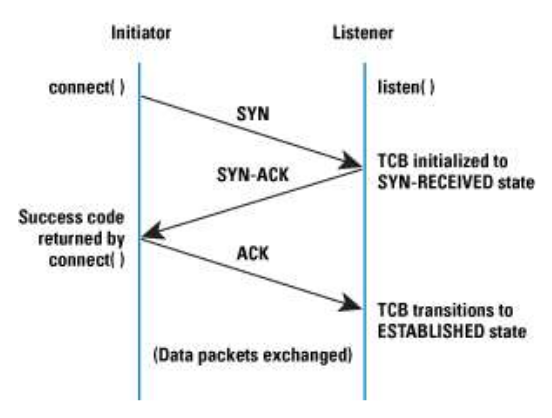
\includegraphics[width=0.5\textwidth]{3wayhandshake.png}\\[1cm]
\end{center}

\section{SYN Flood attack}\index{Index}
A SYN flood attack is a form of denial of service attack in which the attacker, by getting advantage of the TCP three-way handshake, sends a succession of SYN requests to a target server attempting to consume enough resources in order to make it unavailable for answering other legitimate petitions.\vspace{5mm}

The aim of this report is to explain the technical details as well as the procedure followed in order to perform a SYN flood attack implemented with Python and Scapy using VirtualBox machines.\vspace{5mm}

Here is a view of the message flow during a TCP 3-way handshake while performing a SYN flood attack:

\begin{center}
\vfill
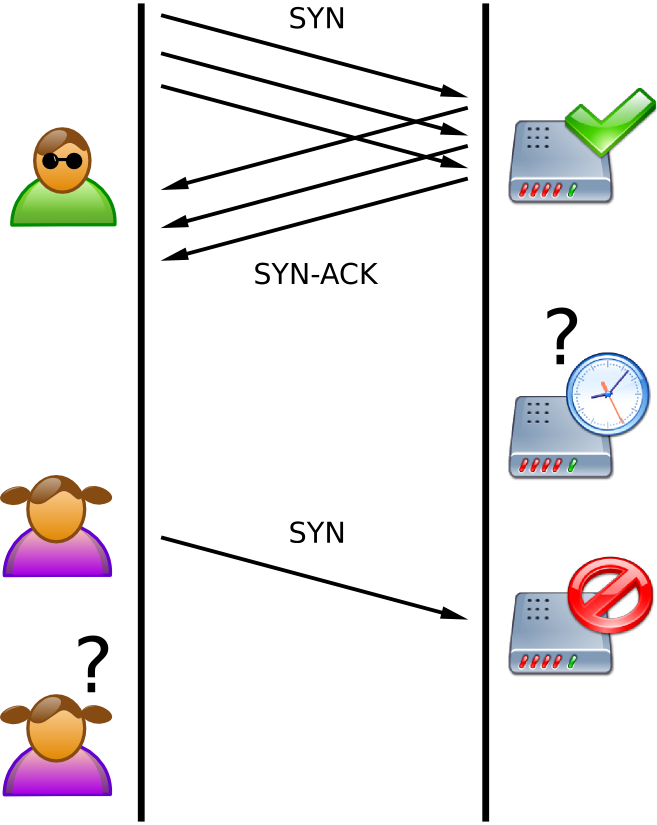
\includegraphics[width=0.5\textwidth]{tcp-synflood.png}\\[1cm]
\end{center}

\clearpage

\section{Why using Scapy}\index{Index}
Scapy is a powerful interactive packet manipulation tool written in Python that allows us to end, sniff and dissect network packets. It is able to forge or decode packets of a wide number of protocols, send them on the wire, capture them, match requests and replies, among other things. It can easily handle most classical tasks like scanning, tracerouting, probing, unit tests, attacks or network discovery.\vspace{5mm}

What's special about Scapy? It does not interpret, it decodes.\vspace{5mm}

Machines are good at decoding and can sometimes help human with that. Interpretation is reserved for human beings. Some programs try to mimic this behavior. For instance they say “this port is open” instead of “I received a SYN-ACK”. Sometimes they are right. Sometimes they are not. It might be easier for beginners, but when you know what you’re doing, you keep on trying to deduce what really happened from the program’s interpretation to make your own, which is hard because you lost a big amount of information.\vspace{5mm}

Moreover, with most other networking tools, you won’t build something the author did not imagine. These tools have been built for a specific goal and can’t deviate much from it. Scapy tries to overcome those problems. It enables you to build exactly the packets you want. Even if I think stacking a 802.1q layer on top of TCP has no sense, it may have some for somebody else working on some product I don’t know. Scapy has a flexible model that tries to avoid such arbitrary limits. You’re free to put any value you want in any field you want and stack them like you want. You’re the adult after all.\vspace{5mm}

In this report, we will be taking advantage of that freedom Scapy offers to craft malformed packets that will be sent to the target server. Since it is written in Python, we will write really simple Python scripts using Scapy as a library to achieve that.
\clearpage

\section{Implementation details of the attack}\index{Index}


\clearpage

\section{Virtual machines' deployment}\index{Index}


\clearpage

\section{Why using iptables to prevent it}\index{Index}


\clearpage

\section{Implementation details of the prevention}\index{Index}


\clearpage

\section{Conclusion}\index{Index}


\clearpage

\section{References and bibliography}\index{Index}

\url{https://www.owasp.org/index.php/Denial_of_Service}\break
\url{https://resources.sei.cmu.edu/asset_files/WhitePaper/1996_019_001_496172.pdf#page=123}\break
\url{http://citeseerx.ist.psu.edu/viewdoc/download?doi=10.1.1.206.5378&rep=rep1&type=pdf}\break
\url{https://en.wikipedia.org/wiki/SYN_flood}\break
\url{https://scapy.readthedocs.io/en/latest/introduction.html#about-scapy}\break


%----------------------------------------------------------------------------------------
\printindex
\end{document}
